\chapter{Evaluation and Preconditioning of the \texorpdfstring{$\wdtnv$}{w-dTNV} Prior}
\label{app:wdtnv_details}

\section{Closed-Form Inverse Square Root for Two Modalities}
\label{app:inv_sqrt_2x2}

For $M=2$, $\Omegaeps{\mathcal{G}}$ of~\eqref{eq:spectral_weight} can be evaluated without an eigendecomposition. Following Chapter~\ref{chapter:wdtnv}, we suppress the voxel index and image dependence of the local Jacobian. Let $\bm{g}_1,\bm{g}_2$ be the columns of $\mathcal{G}\in\mathbb{R}^{d\times2}$ and write
\begin{equation}
    \begin{aligned}
    G_\epsilon:=\mathcal{G}^\top \mathcal{G}+\epsilon^2\mathbb{I}
    &=
    \begin{pmatrix}
    \|\bm{g}_1\|_2^2+\epsilon^2 & \langle \bm{g}_1,\bm{g}_2\rangle\\
    \langle \bm{g}_1,\bm{g}_2\rangle & \|\bm{g}_2\|_2^2+\epsilon^2
    \end{pmatrix},\\
    t&:=\operatorname{tr}(G_\epsilon),
    \qquad
    \delta:=\sqrt{\det(G_\epsilon)}.
    \end{aligned}
\end{equation}
Since $\mathcal{G}^\top \mathcal{G}\succeq0$ and $\epsilon>0$, $G_\epsilon$ is positive definite and $\delta>0$. The Cayley--Hamilton theorem gives $G_\epsilon^2-tG_\epsilon+\delta^2\mathbb{I}=0$, and hence
\[
(G_\epsilon+\delta\mathbb{I})^2=(t+2\delta)\,G_\epsilon.
\]
Since $G_\epsilon+\delta\mathbb{I}$ is positive definite, the principal square-root of $G_\epsilon$ is
\[
G_\epsilon^{1/2}=\frac{G_\epsilon+\delta\mathbb{I}}{\sqrt{t+2\delta}}.
\]
Inverting with the $2\times2$ adjugate formula, using $\det(G_\epsilon+\delta\mathbb{I})=\delta(t+2\delta)$, yields
\begin{equation}
    \Omegaeps{\mathcal{G}}
    =G_\epsilon^{-1/2}
    =\frac{(t+\delta)\,\mathbb{I}-G_\epsilon}{\delta\sqrt{t+2\delta}}.
    \label{eq:inv_sqrt_2x2}
\end{equation}
Each voxel therefore requires three dot products and two scalar square-roots.

\section{Assembly of the Lewis--Sendov Voxel Blocks}
\label{app:ls_block_assembly}

The block approximation used in Chapter~\ref{chapter:optimisation} retains PET/SPECT coupling within each voxel and omits coupling between voxels. The following construction specifies how the local derivatives are assembled into those approximate blocks.

For a local weighted directional Jacobian $\mathcal{G}\in\mathbb{R}^{d\times M}$, write $G=\mathcal{G}^\top \mathcal{G}=V\operatorname{diag}(\lambda_i)V^\top$ and $s_i=\sqrt{\lambda_i+\epsilon^2}$. Equation~\eqref{eq:phi_gram_spectral} expresses $\phi$ as a spectral function of $G$, to which the Lewis--Sendov Hessian formula applies \cite[Theorem~3.3]{doi:10.1137/S089547980036838X}. Applying the chain rule gives the following equivalent expression for the Jacobian-space Hessian acting on a perturbation $E\in\mathbb{R}^{d\times M}$:
\begin{equation}
    \begin{aligned}
    \nabla^2\phi(\mathcal{G})[E]
    &=E\,\Omegaeps{\mathcal{G}}
    +\mathcal{G}V\left[K\circ\left(V^\top(\mathcal{G}^\top E+E^\top \mathcal{G})V\right)\right]V^\top,\\
    K_{ij}&=-\frac{1}{s_i s_j(s_i+s_j)}.
    \end{aligned}
    \label{eq:ls_local_hessian_action}
\end{equation}
Here $\circ$ denotes the Hadamard product. The first term differentiates the explicit factor $\mathcal{G}$ in $\nabla\phi(\mathcal{G})=\mathcal{G}\Omegaeps{\mathcal{G}}$; the second accounts for the change in $\Omegaeps{\mathcal{G}}$. For distinct eigenvalues, $K_{ij}$ is the divided difference $(s_i^{-1}-s_j^{-1})/(\lambda_i-\lambda_j)$. The displayed form also covers repeated eigenvalues, where $K_{ij}=-1/(2s_i^3)$, and zero eigenvalues, since $\epsilon>0$.

Let $E_{\ell m}$ be the $d\times M$ matrix with a single unit entry in difference channel $\ell$ and modality $m$. The direction-diagonal local block retained at target $r$ is
\begin{equation}
    [\Theta_{r,\ell}]_{mm'}
    =\left\langle E_{\ell m},\,
    \nabla^2\phi(\tilde{\mathcal G}_r)[E_{\ell m'}]\right\rangle_F,
    \qquad m,m'=1,\ldots,M,
    \label{eq:ls_local_direction_block}
\end{equation}
where $\langle A,B\rangle_F=\operatorname{tr}(A^\top B)$. For PET/SPECT, $M=2$, so this is a $2\times2$ block.

In practice each voxel block is assembled per neighbourhood target: the Lewis--Sendov calculus is evaluated in local Jacobian coordinates, and the retained direction-diagonal blocks are mapped into modality space by the diagonal congruence
\begin{equation}
    T_{r,\ell}
    =
    \operatorname{diag}(a_{r,\ell})\,
    \Theta_{r,\ell}\,
    \operatorname{diag}(a_{r,\ell})
    =
    \bigl(a_{r,\ell}a_{r,\ell}^{\top}\bigr)\circ \Theta_{r,\ell},
    \label{eq:ls_block_pullback}
\end{equation}
where $\Theta_{r,\ell}$ is the local Hessian block for difference channel $\ell$ at target $r$ and the modality scalings $[a_{r,\ell}]_m$ combine the modality weights $\rho_{m,r}$ and the stencil step scaling with the square roots of the channel-$\ell$ diagonal entries of the operator Gram matrices $\Pi_{m,r}^{\top}\Pi_{m,r}$. Each contribution~\eqref{eq:ls_block_pullback} is the Hadamard product of a rank-one Gram matrix with a positive-semidefinite local block---$\Theta_{r,\ell}$ is a principal block of the local Hessian of the convex smoothed spectral penalty---hence positive semidefinite by the Schur product theorem. Accumulated over the targets incident on voxel $n$ and their difference channels, the assembled voxel blocks are therefore positive semidefinite before flooring. Because the scalings compress the cross-operator geometry to its diagonal energies, the assembled blocks approximate the exact voxel blocks $[H_{\widetilde{\mathcal R}}]_{nn}$ rather than reproducing them exactly.

\section{Majorisation--Minimisation Preconditioners}
\label{app:mm_preconditioner}

Chapter~\ref{chapter:optimisation} builds its prior-curvature models from the Lewis--Sendov Hessian of \wdtnv. This section describes an alternative built from a quadratic majoriser of the prior. It is not used in Chapter~\ref{chapter:paper}, but its diagonal form was used for the subset experiment (Section~\ref{sec:optimisation_subset_selection}).

\subsection{Construction}

Let $\mathcal{G}\in\mathbb{R}^{d\times M}$ and let $\mathcal{G}_0\in\mathbb{R}^{d\times M}$ be a reference Jacobian. Let $\phi(\mathcal{G})=\sum_{i}g(\sigma_i(\mathcal{G}))$ with $g$ the Charbonnier function of Chapter~\ref{chapter:wdtnv}, and let $C_0=\Omegaeps{\mathcal{G}_0}$. Then
\begin{equation}
    \phi(\mathcal{G})
    \leq
    \phi(\mathcal{G}_0)
    +\tfrac12\operatorname{tr}\!\left[\left(\mathcal{G}^\top \mathcal{G}-\mathcal{G}_0^\top \mathcal{G}_0\right)C_0\right],
    \label{eq:jacobian_majoriser}
\end{equation}
with equality at $\mathcal{G}=\mathcal{G}_0$. Since $\phi(\mathcal{G})=\operatorname{tr}((\mathcal{G}^\top \mathcal{G}+\epsilon^2\mathbb{I}_M)^{1/2})-M\epsilon$ and the matrix square root is operator concave \cite{bhatiaMatrixAnalysis1997a}, $\phi$ is a concave function of the Gram matrix $\mathcal{G}^\top \mathcal{G}$, and~\eqref{eq:jacobian_majoriser} is its tangent bound. For $M=1$, $C_0$ is the familiar \gls{irls} weight for the Charbonnier potential \cite{fessler_image_2017,charbonnier_deterministic_1997}. It is also the same inverse square root that evaluates the prior gradient in Chapter~\ref{chapter:wdtnv}.

Summing~\eqref{eq:jacobian_majoriser} over voxels, with $\mathcal{G}_0$ the weighted directional Jacobian $\tilde{\mathcal G}_n$ at a preconditioner refresh, gives a quadratic majoriser of the prior. Its Hessian couples neighbouring voxels, so, as for the Lewis--Sendov models, only voxel blocks are retained. Writing $C_r=\Omegaeps{\tilde{\mathcal G}_r}$ at target voxel $r$, the voxel block of this Hessian is
\begin{equation}
    \widehat H_{\widetilde{\mathcal R},n}^{\mathrm{MM\text{-}block}}
    =
    V_{\mathrm{vox}}
    \sum_{r\in\mathcal N(n)}
    \left[B_rC_rB_r\right]\circ A_{r\leftarrow n},
    \qquad
    [A_{r\leftarrow n}]_{mm'}
    =
    c_{r\leftarrow n}^\top\Pi_{m,r}^\top\Pi_{m',r}c_{r\leftarrow n},
    \label{eq:mm_block_preconditioner}
\end{equation}
where $\mathcal N(n)$ is the set of target voxels whose finite-difference stencil contains $n$, $c_{r\leftarrow n}$ is the response at $r$ of the difference operator to a unit impulse at $n$, $B_r=\operatorname{diag}(\rho_{1,r},\rho_{2,r})$, and $\circ$ is the Hadamard product. The \emph{Jacobi diagonal} keeps the diagonal of each block.

If valid data and prior majorisers are built at a common anchor, their curvatures add, and the inverse sum~\eqref{eq:parallel_sum_combination} is the corresponding \gls{mm} step. Extracting voxel blocks or diagonals from the spatially coupled Hessian does not preserve the majorisation, however, so none of these models is a global majoriser and the interpretation is heuristic.

\subsection{Cost and Comparison}

Construction and cached application of the two block models were timed on an NVIDIA RTX 3080 using ten repeats after two warm-up evaluations, for the one-bed phantom and two-bed patient configurations (Table~\ref{tab:mm_preconditioner_cost}). Application costs the same for both, but \gls{mm} construction is cheaper: Lewis--Sendov construction took 51\% and 72\% longer for one and two beds. This reflects the work each needs: the \gls{mm} block needs only the $2\times2$ inverse square root $C_r$ at each target, whereas the Lewis--Sendov block needs voxel-wise singular-value decompositions and the spectral Hessian terms built from them. Using the Chapter~\ref{chapter:paper} subset counts (18 PET plus 12 SPECT for one bed, or 36 PET plus 12 SPECT for two beds), with one construction and 30 or 48 applications per epoch, application dominates and the saving is small: approximately $8.2$ versus $8.5\,\mathrm{s}$ per epoch for one bed, and $55.7$ versus $58.3\,\mathrm{s}$ for two beds.

\begin{table}[htbp]
    \centering
    \caption{Mean construction and cached application times in seconds for the two block preconditioners; uncertainties are standard deviations over ten repeats.}
    \label{tab:mm_preconditioner_cost}
    \small
    \begin{tabular}{@{}llrr@{}}
        \toprule
        Preconditioner & Operation & One bed & Two beds\\
        \midrule
        \multirow{2}{*}{\gls{mm} block}
            & Construction & $0.920 \pm 0.0149$ & $3.416 \pm 0.0259$\\
            & Application  & $0.242 \pm 0.0019$ & $1.090 \pm 0.0046$\\
        \addlinespace
        \multirow{2}{*}{Lewis--Sendov block}
            & Construction & $1.389 \pm 0.0141$ & $5.867 \pm 0.0395$\\
            & Application  & $0.237 \pm 0.0011$ & $1.093 \pm 0.0052$\\
        \bottomrule
    \end{tabular}
\end{table}

\begin{figure}[htbp]
    \centering
    \begin{subfigure}{0.93\linewidth}
        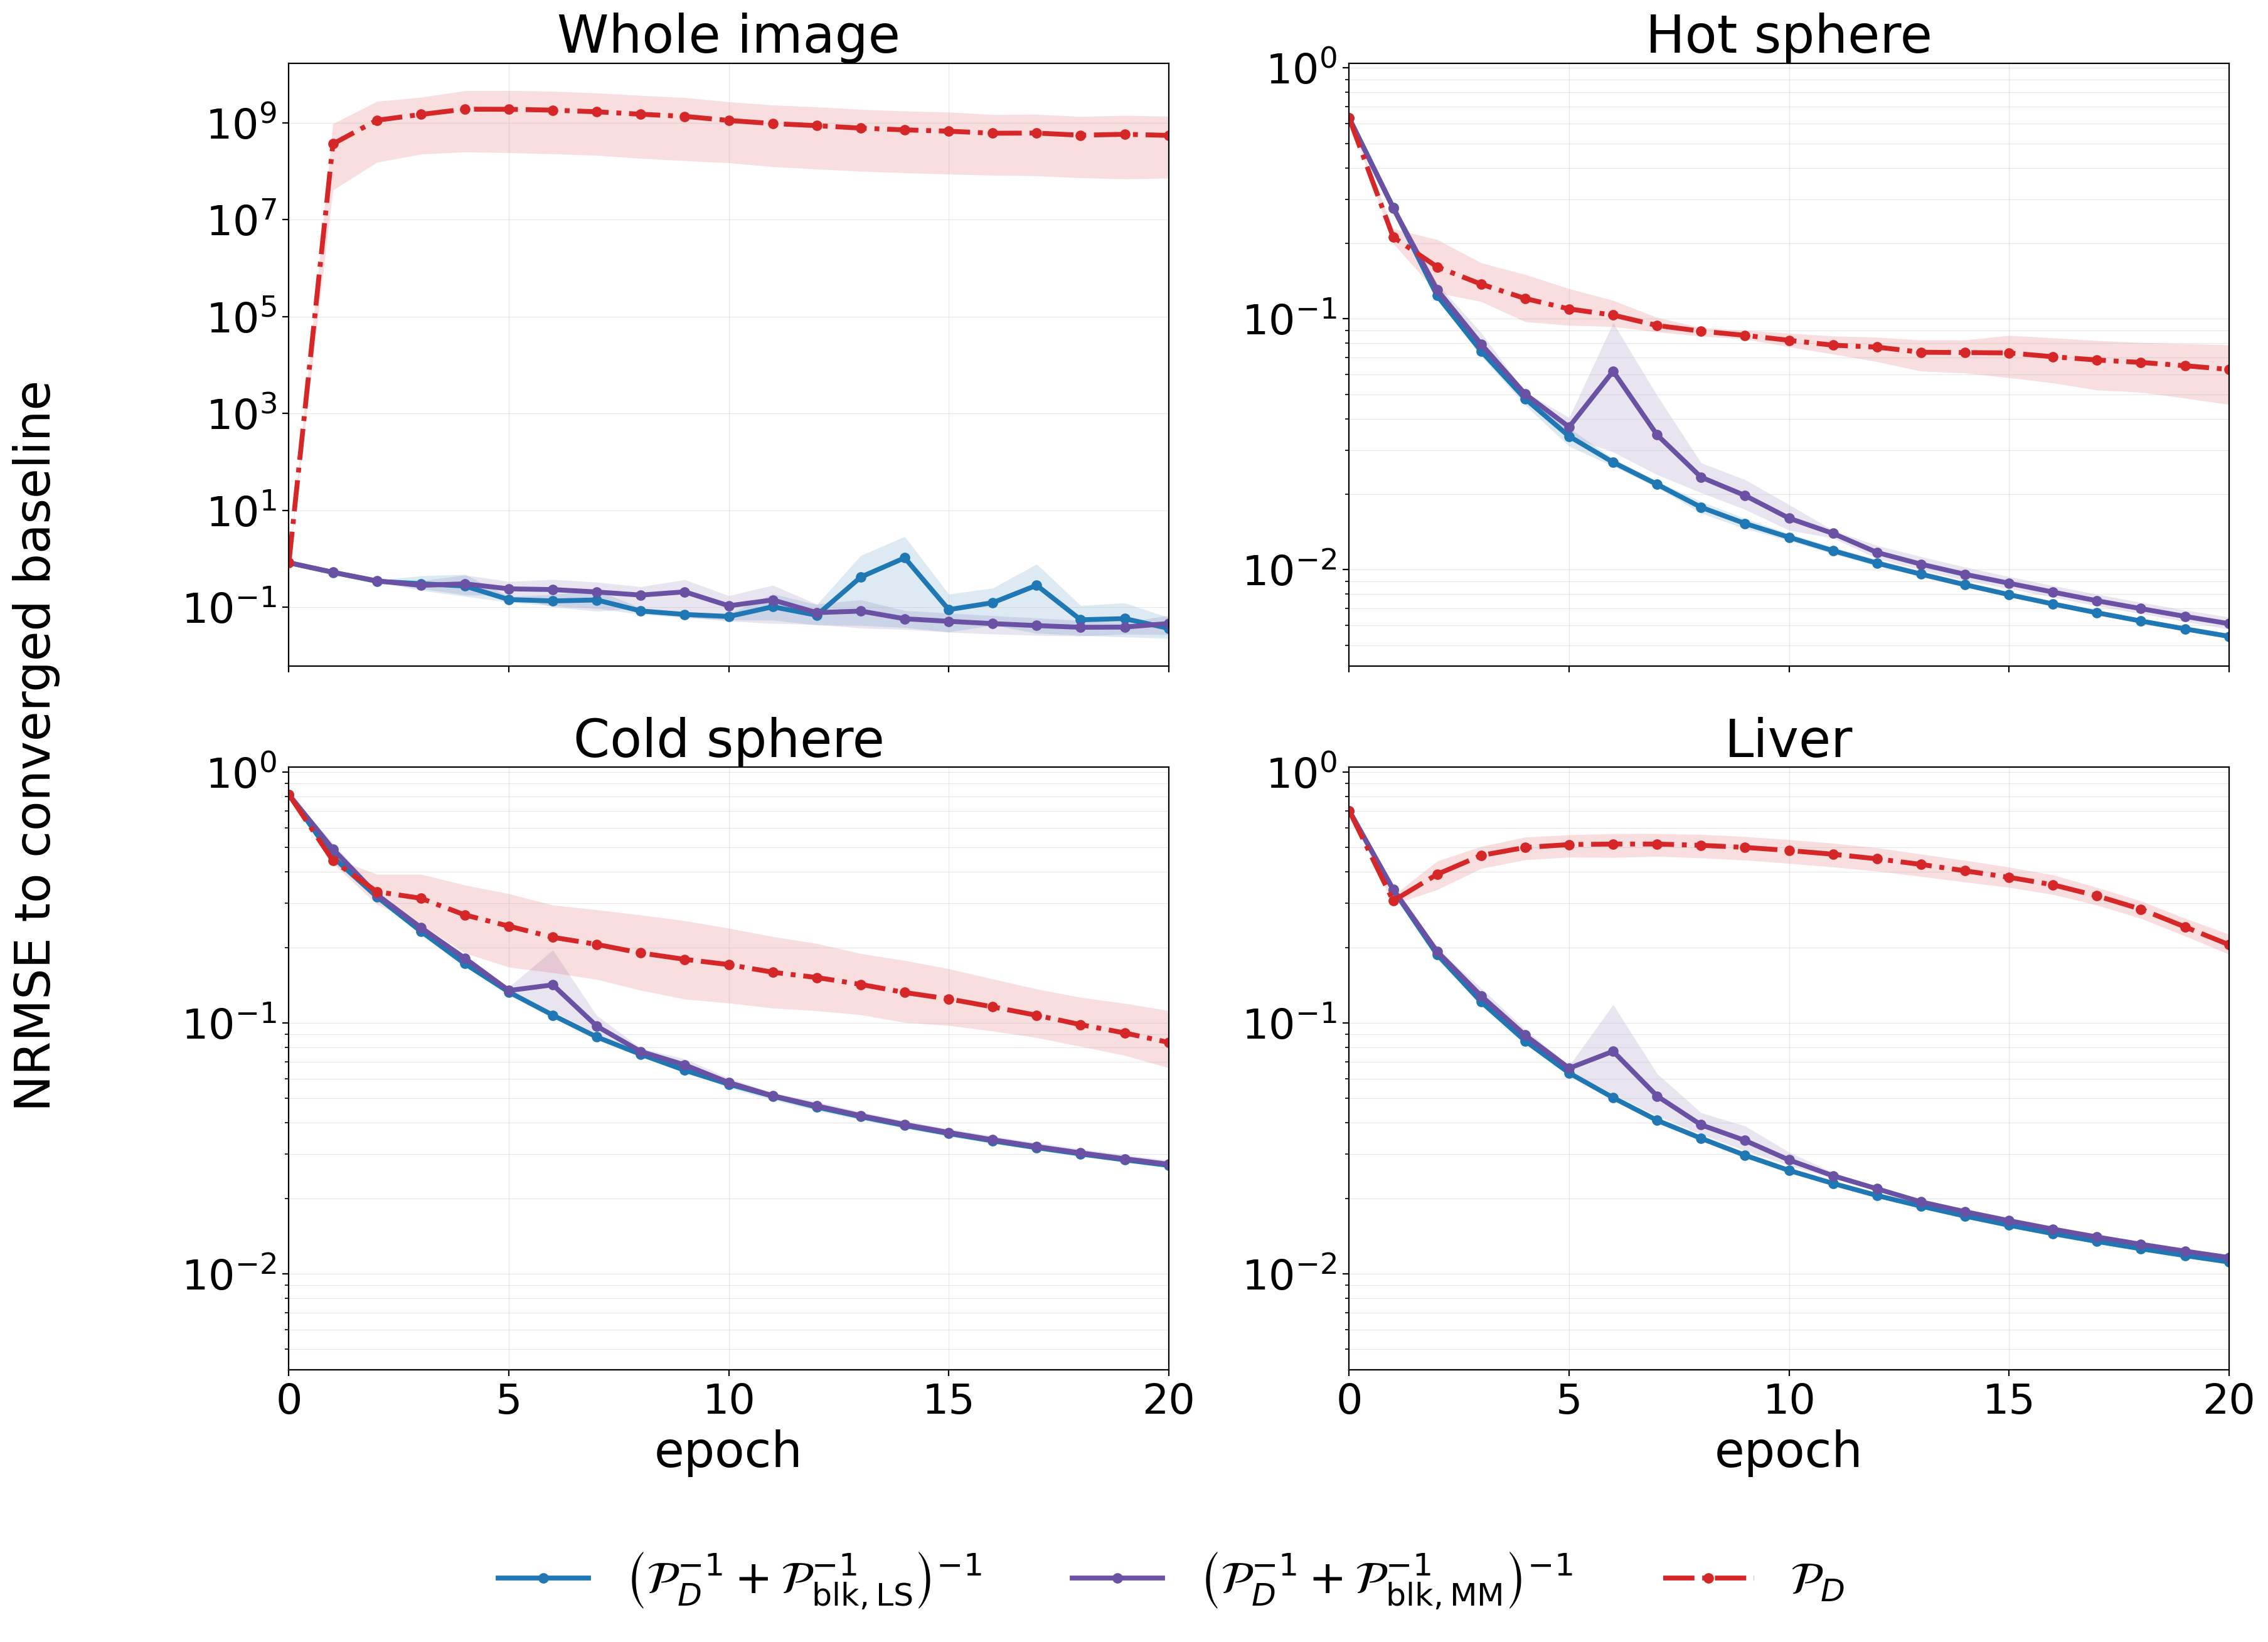
\includegraphics[width=\linewidth]{figures/preconditioning/ls_vs_mm_blk/exp3_best_precond_1bpos.png}
        \caption{\gls{pet}.}
    \end{subfigure}
    \begin{subfigure}{0.93\linewidth}
        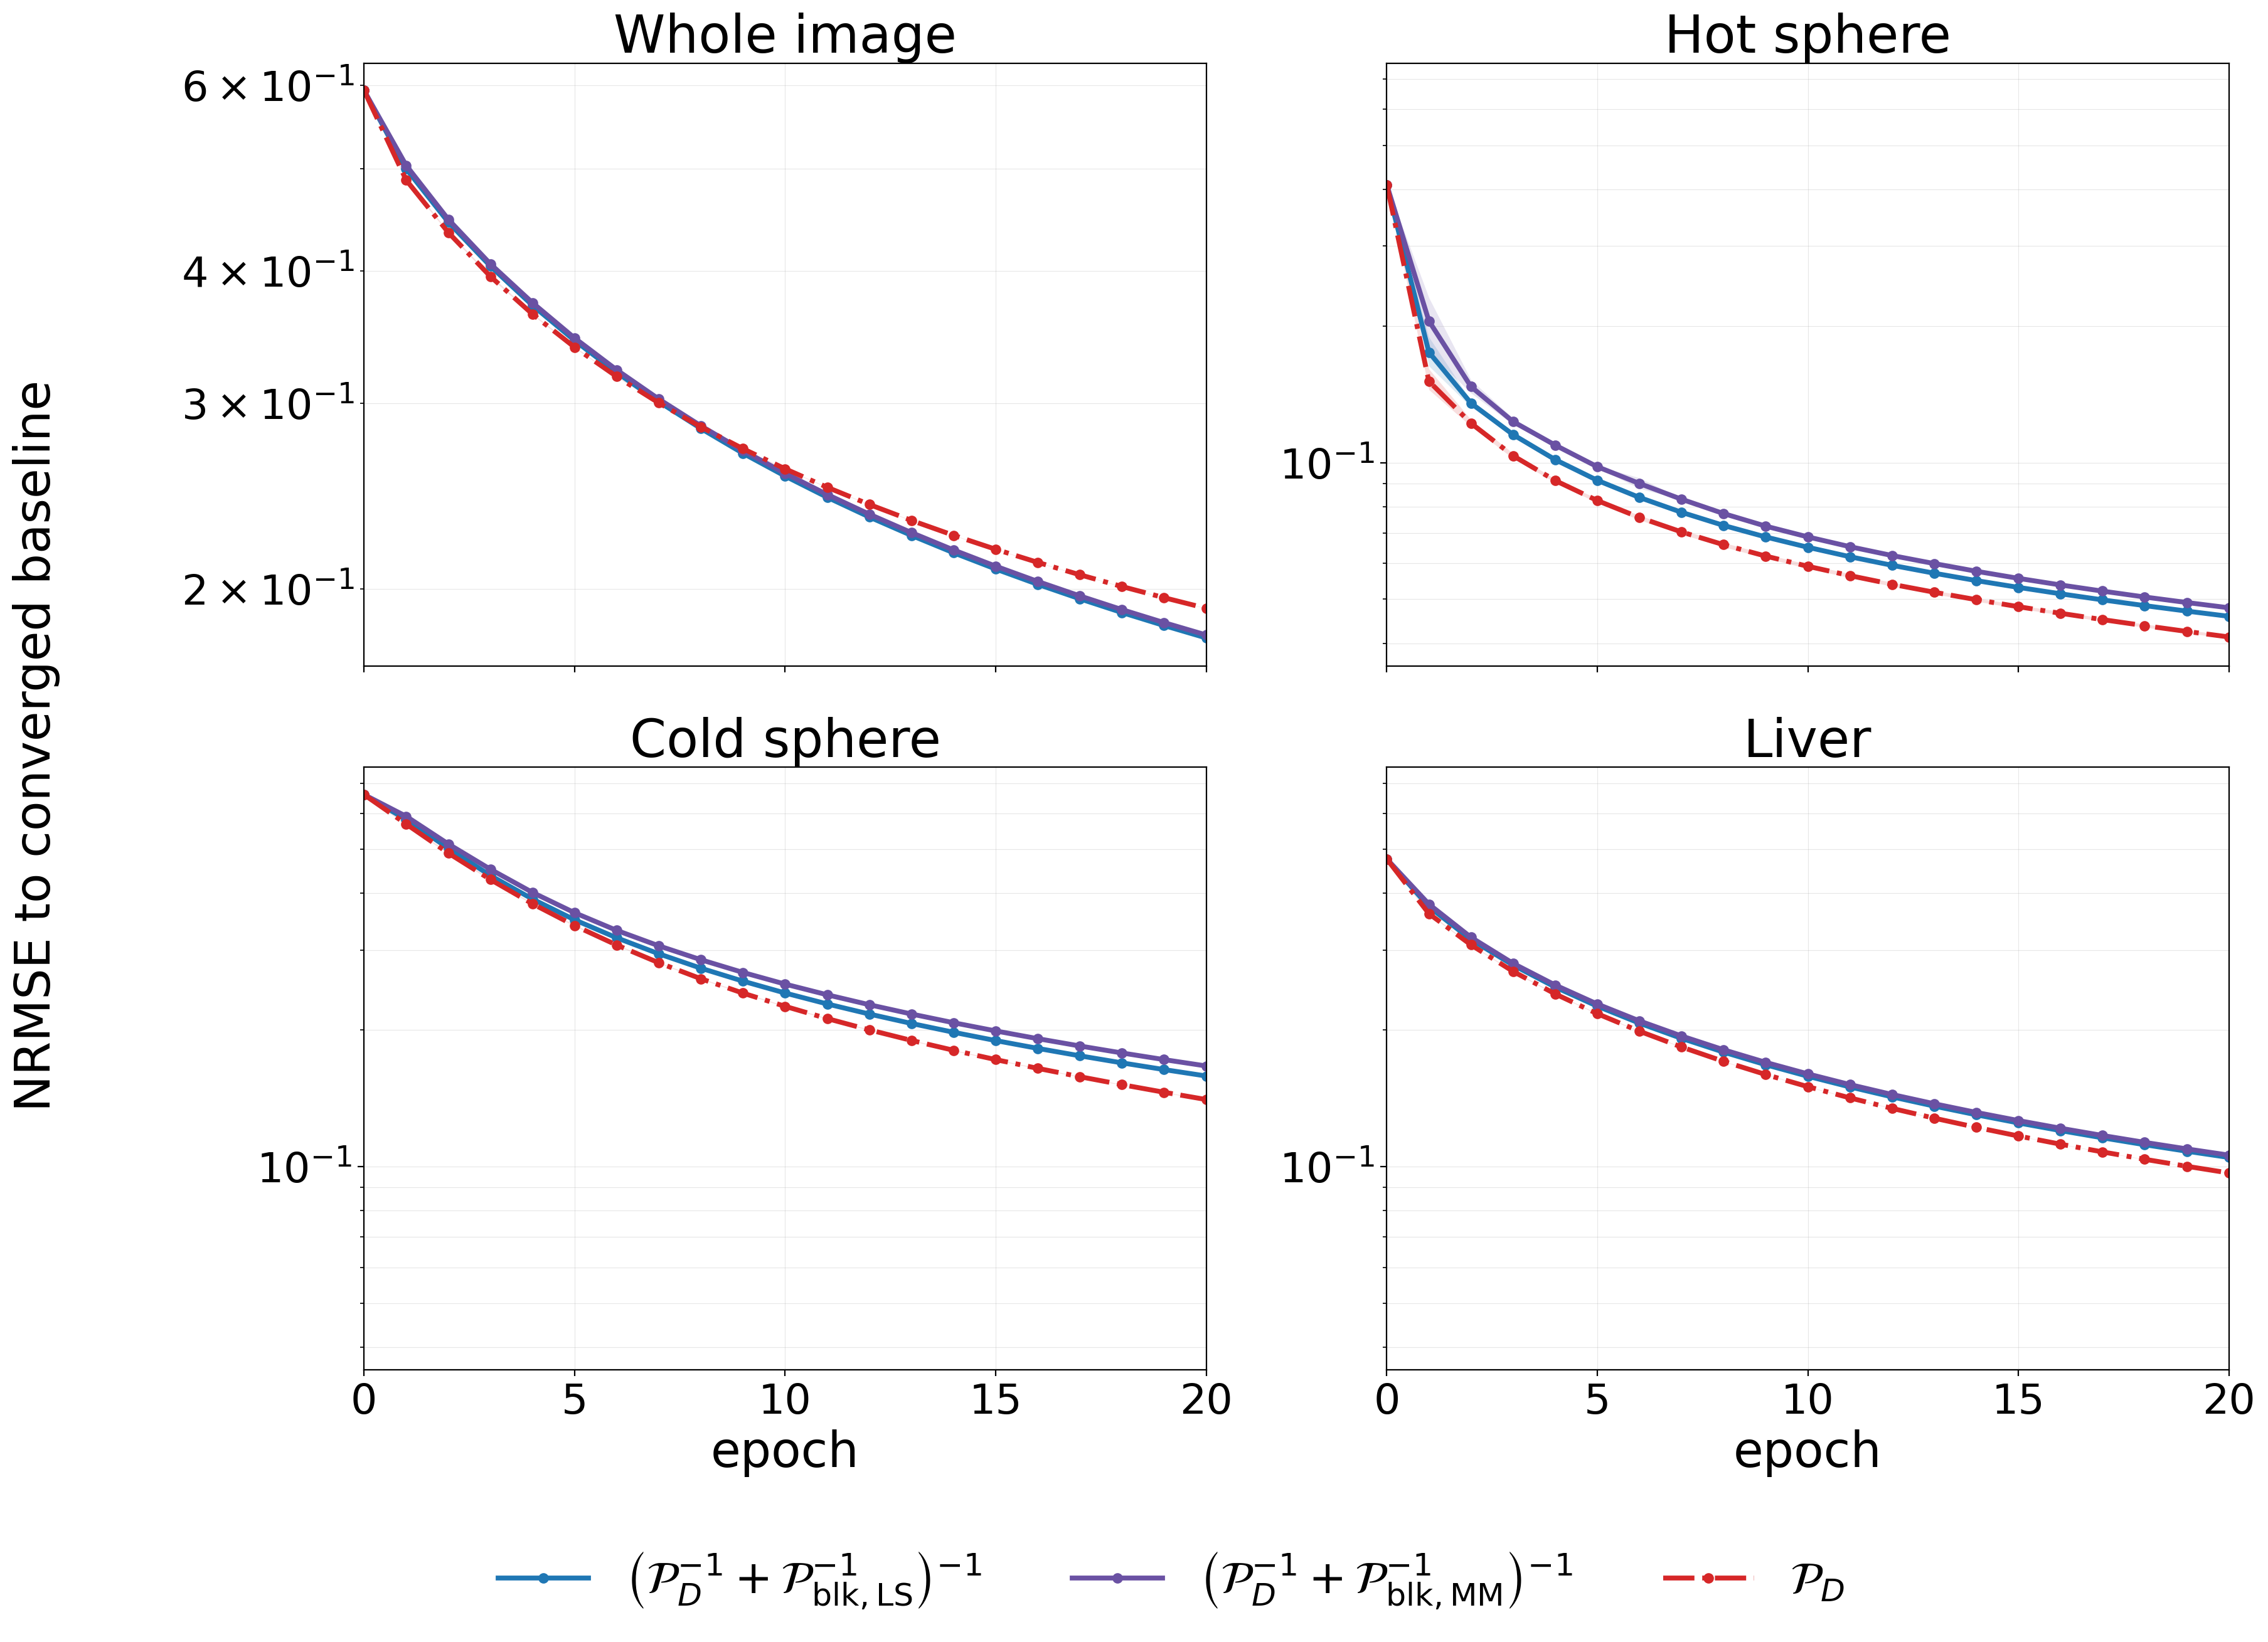
\includegraphics[width=\linewidth]{figures/preconditioning/ls_vs_mm_blk/exp3_best_precond_1bpos_SPECT.png}
        \caption{\gls{spect}.}
    \end{subfigure}
    \caption{\gls{nrmse} trajectories for the inverse-sum combinations of data-only scaling with the Lewis--Sendov ($\mathcal P_{\mathrm{blk,LS}}$) and \gls{mm} ($\mathcal P_{\mathrm{blk,MM}}$) block prior models, with data-only \gls{bsrem} ($\mathcal P_{\mathcal D}$, labelled $\mathcal P_D$ in the panels) for reference. Lines and shading show the five-run mean and pointwise minimum--maximum over 20 matched expected data-draw units.}
    \label{fig:mm_vs_ls_block}
\end{figure}

Under the protocol of Section~\ref{subsec:preconditioner_experiment_methods}, the two block models gave similar \gls{nrmse} (Figure~\ref{fig:mm_vs_ls_block}). The Lewis--Sendov block was slightly lower in most anatomical regions. The \gls{mm} block showed a transient increase near pass 6 in the \gls{pet} anatomical regions, and the Lewis--Sendov block showed transient whole-image increases near passes 14 and 17. With similar convergence and cheaper construction, the \gls{mm} block is a reasonable alternative where construction cost matters.
